\chapter{项目内容及优化实现}\label{sec:algorithm}

本章介绍了项目在准备阶段和项目各部分优化细节。项目的准备阶段包括数据库的设计与实施、系统代码的编写以及短视频压缩编码的初步实现。优化细节包括数据库性能瓶颈分析与消除、数据库语句优化以及视频压制优化。

\section{数据库的设计}
 
\subsection{需求分析}
设计数据库首先要进行需求分析\cite{gamma1995design}。本系统需要数据库来管理与储存用户信息、视频信息、视频的评论信息用户以及用户与视频的各种关系。用户信息包含用户的系统内唯一编号、用户名、密码、注册时间、用户头像以及用户各项统计信息等内容。视频信息包括视频名称、视频文件存放位置、视频作者、视频相关统计信息等内容。评论信息包含评论人、评论内容、评论种类、评论视频等内容。用户与视频关系包含关系类型、用户编号与视频编号等内容。

为了需求分析的简便,我们先将用户与视频所有的信息放入一张表中,其 E-R 图如图 \ref{fig:ER1} 所示。随后我们要进行关系的规范化。

\begin{figure}[!ht]
    \centering
    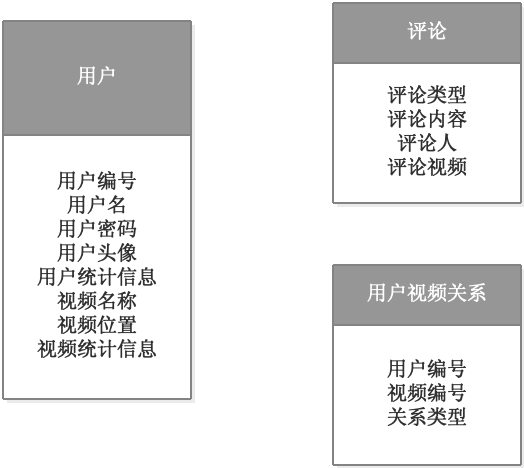
\includegraphics[width=0.5\textwidth]{dbs1.png}
    \caption{需求分析数据库 E-R 图}
    \label{fig:ER1}
\end{figure}


\subsection{关系规范化}

经过初步地需求分析后,我们得到了一个初步地数据库模型,但这个模型仅仅遵循了关系数据库理论的第一范式\cite{codd1972further},即所有的属性均为原子属性。仅遵循第一范式的模型有插入异常、删除异常以及修改复杂等缺点。以此模型中的用户表为例。当一个用户没有任何视频时无法将该用户插入,导致更新异常。当一个用户信息需变更时需改变所有包含用户信息的元组,导致修改复杂。当用户删除所有视频时会导致用户信息被一同删除,导致删除异常。

为了解决这些问题,我们需要使数据库符合第二范式\cite{codd1972further},即关系遵循第一范式,且关系中所有的非主属性都完全函数依赖于任何候选码。为了使关系遵循第二范式,我们要对其进行规范化,即将一个大的关系拆分为两个或多个小的关系。我们将用户表拆分为用户信息表和视频信息表,两个表的函数依赖关系在拆分后由外健保留,关系拆分后 E-R 图 (省略实体的属性) 如图 \ref{fig:ER2} 所示 。

\begin{figure}[!ht]
    \centering
    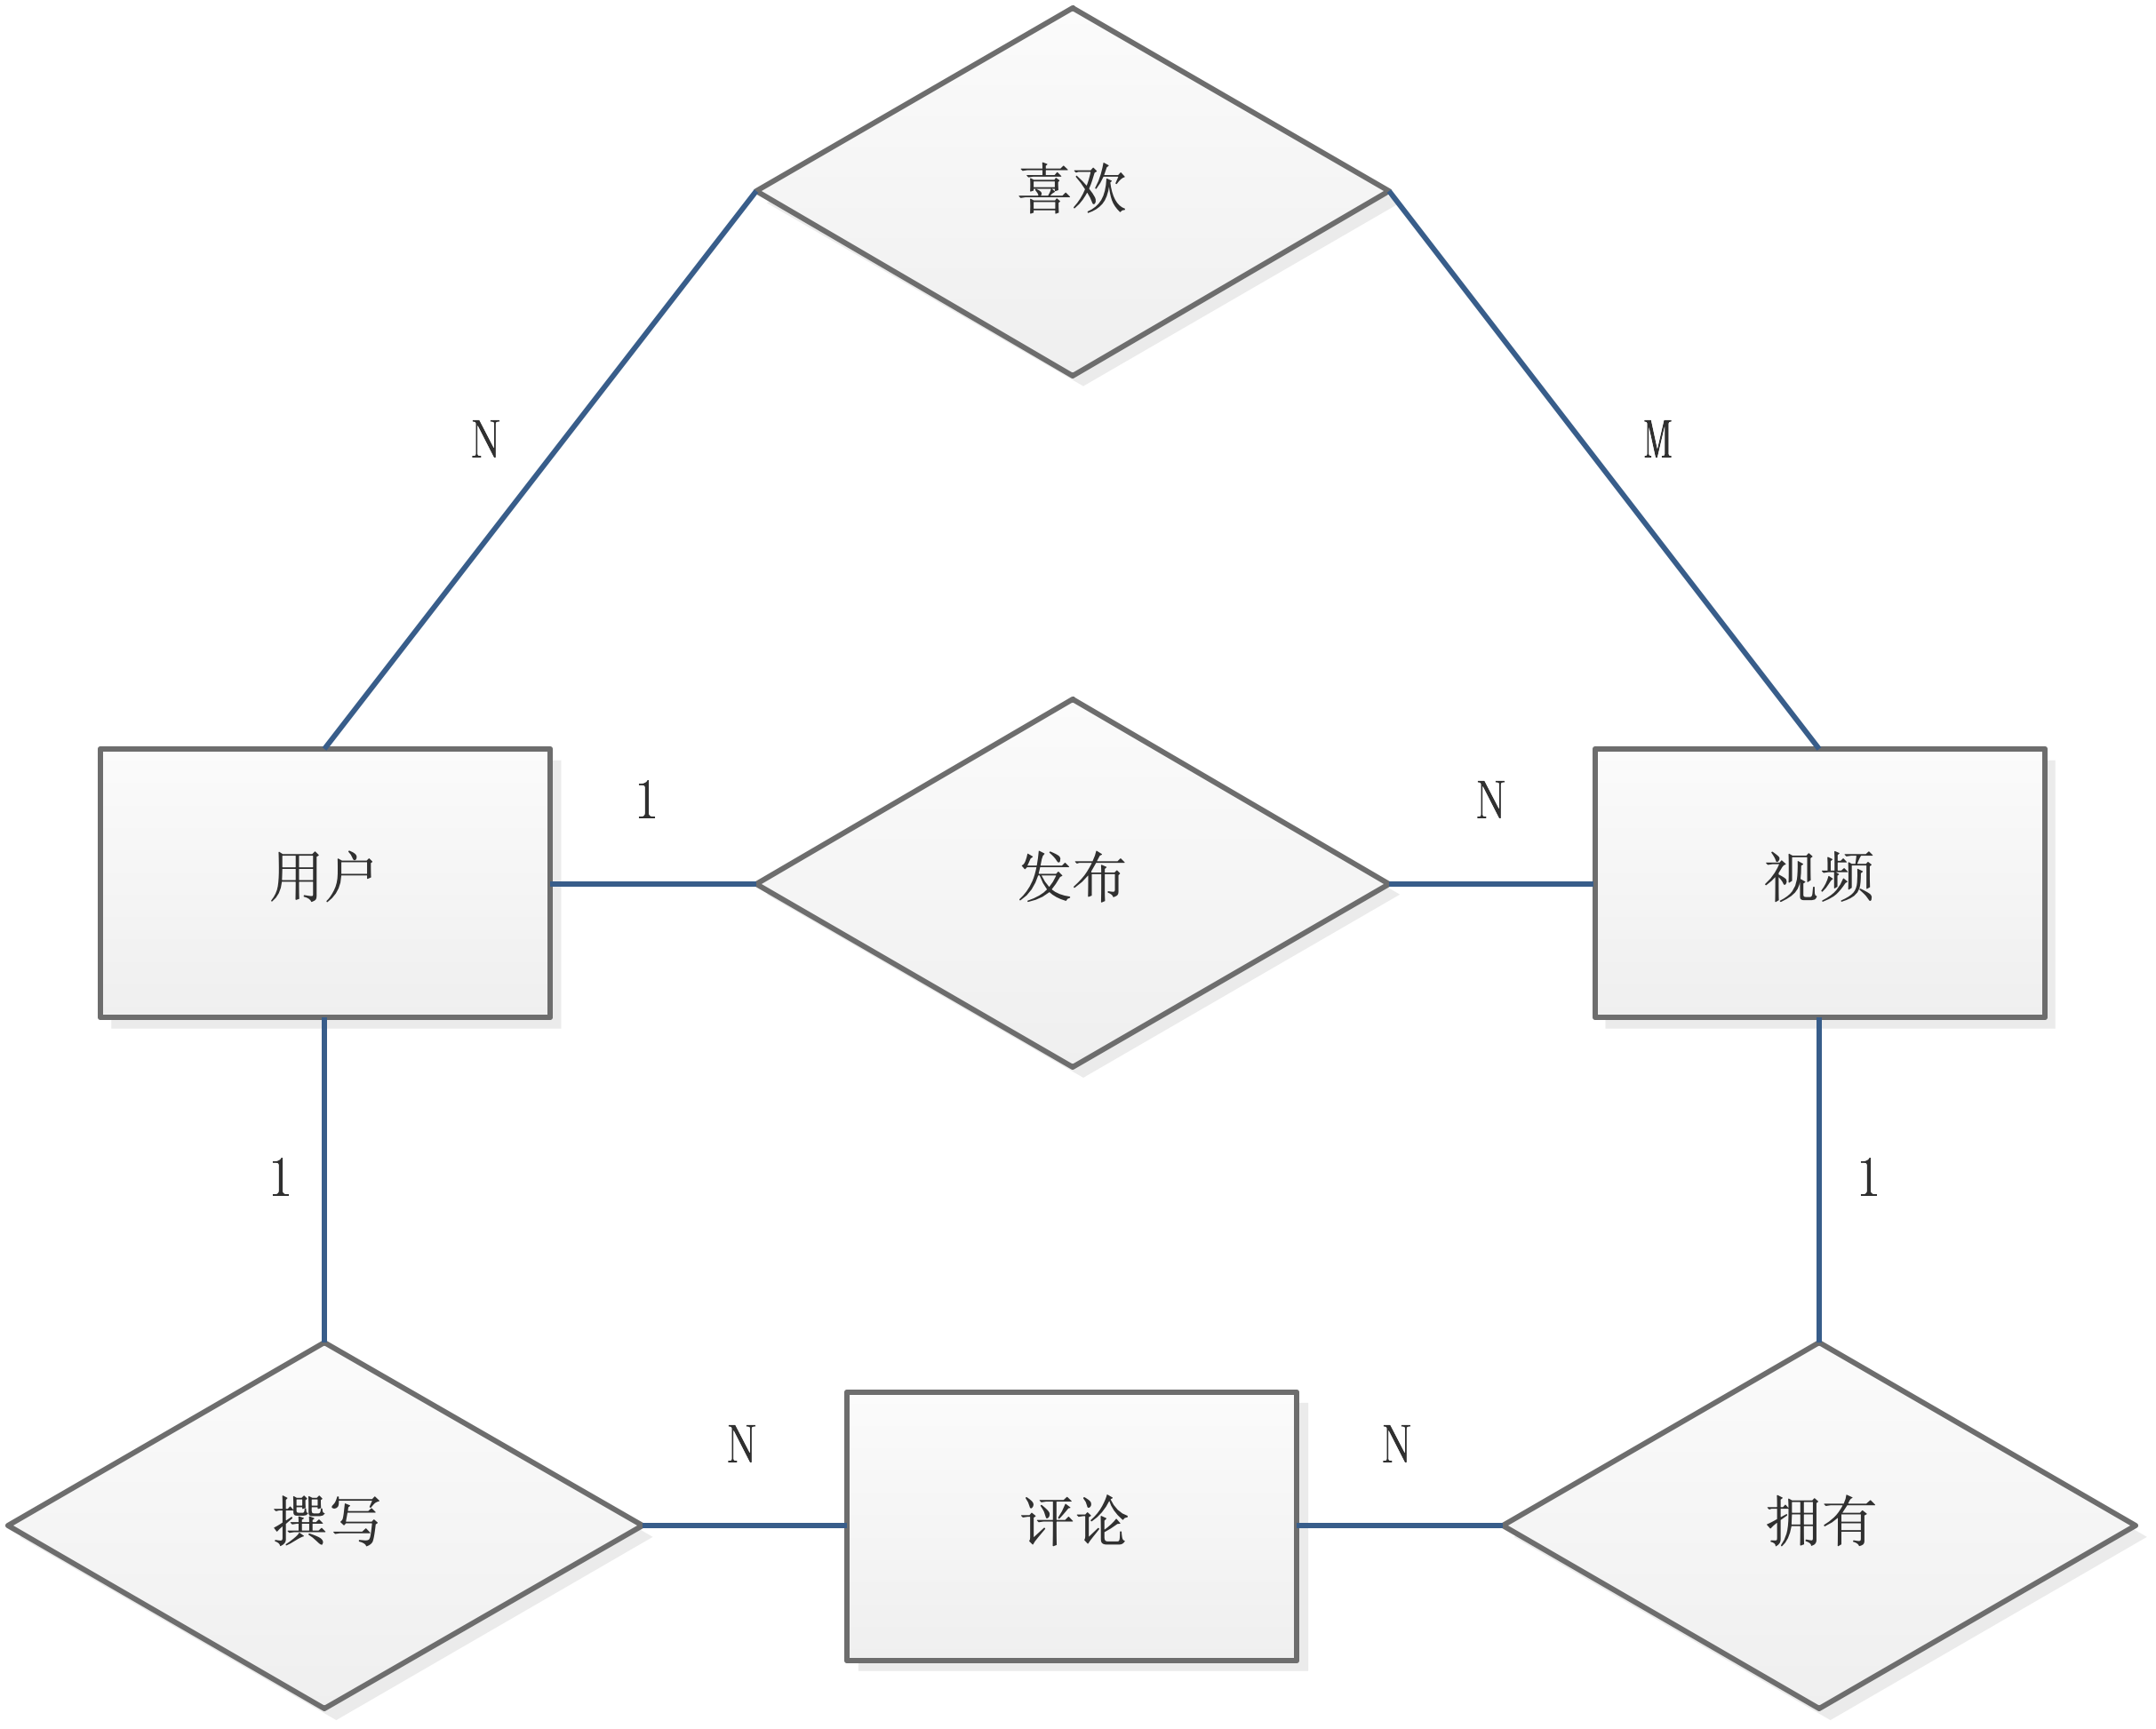
\includegraphics[width=0.6\textwidth]{dbs2.png}
    \caption{规范化后数据库 E-R 图}
    \label{fig:ER2}
\end{figure}

经过关系分解后,用户表与视频表中即不存在关于主属性的传递函数依赖,也不存在非主属性决定子,所以分解后整个关系达到了 BCNF\cite{bernstein1976synthesizing},解决了之前可能出现的问题。

\subsection{数据库逻辑结构设计}

完成数据库的概念结构 (E-R 模型) 后开始设计数据库逻辑结构\cite{gamma1995design}。这里我采用将 E-R 模型转换为关系模型的方法设计数据库逻辑结构。首先以 E-R 模型中各个实体为基础创建关系模式,然后创建实体间的联系。用户与视频间的发布联系是一个一对多联系,将其与 n 端对应的模式即视频关系模式合并。用户与视频间的关系为多对多关系,需单独设置一个关系模式储存。用户与评论以及视频与评论间的联系是一个多元联系,需单独设置一个关系模式\cite{王珊2006数据库系统概论}储存。

本系统使用的关系模式为:用户模式(\uline{用户编号},用户名,用户密码,用户头像,用户统计信息)、视频模式(\uline{视频编号},视频名称,视频位置,视频作者,视频统计信息)、用户与视频间关系模式(\uline{用户编号},\uline{视频编号},关系类型)、用户、视频与评论关系(\uline{评论编号},用户编号,视频编号,评论类型,评论内容)。

\subsection{数据库物理结构设计与实施}

数据库物理结构由 MySQL 数据库管理系统默认生成,将上述关系模式转换为对应的结构化查询语句,并在 MySQL 中创建出相应的数据库表。完成数据库的实施之后,数据库设计完成。



\section{系统代码编写}

\subsection{系统整体设计}
本系统采用层次化结构进行开发,即将系统的功能由底至顶划分为若干层次,各层之间只能逐层单向调用,只能高级层次模块调用低级层次模块,系统各层次之间只提供相应接口,同时将具体实现屏蔽,这样增大了系统各模块内部的内聚度,减小了模块之间的耦合度,有利于系统开发。

\begin{figure}[!ht]
    \centering
    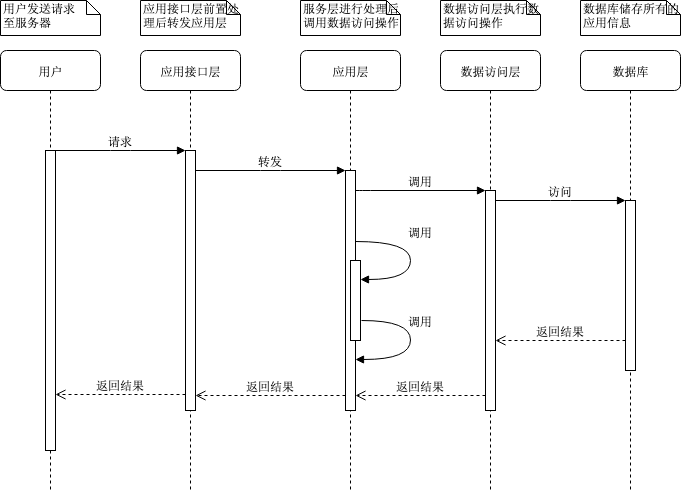
\includegraphics[width=0.6\textwidth]{soft1.png}
    \caption{短视频系统数据流图}
    \label{figs:soft1}
\end{figure}

根据短视频系统的功能要求,本系统被划分为公用功能层、数据访问层、服务层以及应用接口层。如图 \ref{figs:soft1} 所示,公用功能层是整个系统的最底层,含有许多供上层模块使用的静态依赖。数据访问层包含两部分一部分是数据访问对象模块,负责操作数据库;另一部分是实体对象模块负责保存数据库返回的结构。服务层依赖于数据访问层,它负责接收应用接口层发送的请求,做与数据相关的前期处理,封装相应的数据访问操作,并将结果进行处理后返回应用接口层。应用接口层接收用户请求,并作出权限判断等于前端有关的处理后将请求转发给服务层,接收结果后封装成响应结构返回给用户。

\subsection{系统具体实现}
本系统的应用接口层由 SpringMVC 实现、服务层由 Spring IoC 与 Spring AOP 实现、数据访问层基于 MyBatis 框架与 Spring AOP。

应用接口层包含了系统内所有的应用编程接口 (Application Programming Interface, API)。这些 API 主要可以分为三组:与用户相关的 API、与视频管理相关的 API以及处理用户与视频关系的 API。这些 API 均基于 SpringMVC 的注解式 API 声明。服务层包含了系统最主要的功能实现,主要使用 Spring IoC 提供的依赖注入功能获取数据访问依赖。数据访问层基于 MyBatis 框架,编写相应的实体类和访问接口后即可有 MyBatis 负责相应数据的读取与封装,并且使用 Spring AOP 实现对数据库事务的支持。



\section{短视频压缩编码初步实现实现}

短视频的压制与背景音乐合成由 FFmpeg\cite{ffmpeg2019} 实现。FFmpeg 是一组音视频处理工具的集合。根据短视频应用的特性,我初步地将视频分辨率设为 1920 $\times$ 1080,帧率设置为 30 帧,码率采用 2 Mbps,编码采用 h.264 编码,封装格式采用 Mpeg4,兼容性较好,该压制属性可以保证视频中等清晰。

%\begin{lstlisting}
%ffmpeg -i input.MOV -vcodec h264 -profile:v high -level 5.1 -s 1920x1080 -preset slow -b:v 4M -maxrate 8M -bufsize 4M -r 29.97 output.mp4
%\end{lstlisting}



\section{数据库性能优化}

MySQL 优化是指通过各种方式调整 MySQL 或服务器以提升 MySQL 数据库具体性能表现的过程。数据库优化主要可以分为架构优化、参数优化和 SQL 优化。架构优化指对整个系统架构进行分析重构与优化,通常获得结果最好,但最复杂。参数优化指调整操作系统与数据库的参数设置来进行优化的方法,其效果通过基准测试体现。SQL 优化指针对具体数据库表与查询语句进行工程上的调整,效果通过压力测试体现。本文只关注参数优化和性能优化对数据库的性能提升效果。

\subsection{参数优化}

数据库的参数优化\cite{schwartz2012high}是通过调节操作系统与数据库的参数设置来实现的。参数优化的过程中要遵循的原则有重视数据库记录日志、多次进行数据库瓶颈分析以及注意实现数据库读写的平衡。

对于一个事务序列来说最重要的是其能否成功执行。而事务能否成功执行的关键在于其日志文件能否成功落盘保存。因此日志文件对于事务序列方面的优化起着至关重要的作用。其次,我们需要通过查看数据库的监控信息查找数据库的瓶颈并做针对性优化。最后,为了数据库有一个良好的整体性能,我们需要根据我们的系统实际情况对数据库读写性能进行平衡。

在本系统中,我们可以调节数据库内存缓存的大小,以减小磁盘 I/O 操作,以达到更好地性能。随后,我们可以根据数据库的日志文件进行优化,减少数据库日志文件的刷新,以获得更好地性能。最后可以根据监控数据进行优化,观察监控数据中数据库对各项系统资源的占用情况,若 CPU 是系统瓶颈则可以增大线程池以减小线程创建次数。若磁盘称为瓶颈则可以降低并发以获得更好地性能。

本系统选择将 MySQL 数据库的 InnoDB\cite{姜承尧2011mysql} 储存引擎的 innodb\_buffer\_pool\_size 参数设置为 70\% 内存大小,以达到较好的磁盘性能。然后,将 innodb\_buffer\_pool\_size 属性设置为 4G,减小 MySQL 日志产生数量,提高性能。将 innodb\_flush\_logs\_at\_trx\_commit 属性设置为 0,这样做虽然会减小一定的稳定性但会带来较大的性能提升,本系统不需要太高的一致性,所以可以对其进行更改。最后设置合适的允许连接数、开启慢日志查询以及设置合理地缓存命中率对数据库性能均有明显提升。


\subsection{SQL 优化}

数据库的 SQL 优化主要包括为数据库表选取合适的数据类型、选用合适的索引以及优化查询过程等方面。

\subsubsection{适当的数据类型}

数据类型优化原则有尽可能使用较小的数据类型、使用较简单地数据类型以及避免使用 null。较小的数据类型通常处理起来比较快,同时它们占有较小的磁盘空间、内存以及 CPU 缓存,可以在更短的时钟周期内处理。简单数据类型或数据库提供支持的数据类型处理需要的时钟周期更短,如:数据库内建的日期类型处理比字符串储存日期更快。

本系统中对于数据库表的数据类型优化为将所有的与时间、日期相关的属性数据类型改用数据库内建支持类型。将各种统计信息类型减小范围。

\subsubsection{索引}

索引是查询优化最有效的手段。数据库中常用的索引有 B-Tree\cite{严蔚敏2002数据结构} 索引和哈希索引。B-Tree 索引是在需设置索引的属性列上建立多级 B-Tree,查询时通过多路查询与连续查询快速地查找。B-Tree 索引适用于需精确查询和范围查询的情况。哈希索引指为索引列建立哈希表,查找时直接通过哈希查找查询所需数据。哈希索引适用于精确查询。此外在数据库索引设计中还有以下几种设计情形:多列索引、聚簇索引等。多列索引是将多个属性列一同作为索引元素进行索引,好的多列索引的性能远好于多个单列索引。局促索引指将属性值相同的元组存放于磁盘上的临近位置,可以减小查询时的岑攀访问次数,提高性能。

本系统的优化过程中,我对数据库做如下索引优化:在用户表中只需要使用编号与用户查找元组,故在这两个属性上添加 B-Tree 索引提高查询性能。视频表中需按编号、作者以及视频名称查询,在这三个属性上设置 B-Tree 索引,并在作者以及名称属性上设置聚簇索引以加快查询作者全部视频和全部相同名称视频时的速度。 

\subsubsection{查询过程}

大部分查询优化是通过减少查询过程中产生的中间结果数量来进行的。查询过程中若中间结果较多,系统需要大量的时间来判断这些中间结果是否必要,同时大量的中介结果会占用较多的系统资源。本系统使用的查询优化措施为:优化数据库的计数操作、优化多表连接查询以及优化分页查询。

首先我进行了 MySQL 数据库中 COUNT 函数的优化。COUNT 函数是 MySQL 中用来计算查询结果个数的函数,在系统中十分常用。在 MySQL 中使用索引覆盖扫描即可加速 COUNT 函数的执行速度。随后进行关联查询的优化,确保关联查询的连接列上建有索引即可使用索引加速连接过程。分页查询优化使用覆盖索引扫描然后进行一次连接操作来改善性能。最后是将部分使用临时表的嵌套查询转换为使用连接操作的查询以及为连接变量都加上索引。

\section{视频编码优化}
短视频编码方面的优化主要为编码器选择、视频压制参数设置以及是否采用硬件加速等措施。FFmpeg 用于视频压制的编码其默认为 使用 CPU 进行编码的 X264 编码器,在优化时可以选用支持显卡硬件加速的编码器。通过设置视频压制参数可以改变压制视频的质量与压制时间,最后采用硬件加速即显卡参与视频压制可以显著地提高压制速度,但其缺陷为压制出视频画质略逊于 CPU 编码器。

本文采用的优化措施为:选择支持硬件加速的视频编码器 h264\_videotoolbox、选择视频压制码率为 4Mbps、分辨率为 1920x1080、视频帧率为 29.97 帧、视频 profile 选择为 high、编码器预设选择 medium,这样压制出的视频再大小和画质上处于比较均衡的地位。最后使用 intel 核心显卡作为硬件加速显卡加速压制过程。